\chapter{Extended ICA Algorithms}\label{app:ICA}

\section{Independent Component Analysis}
Independent Component Analysis (ICA) is a method which assume statistical independent, in the EEG signal case, between the sources. With this independence it is possible for ICA to separate the scalp mixture $\mathbf{Y}$ into the sources $\mathbf{X}$ and the mixing matrix $\mathbf{A}$.
\\
Through this section the mathematical concepts of Independent Component Analysis (ICA) will be explained and defined.
\\ \\
Lets set up an situations. We have some measurements that has been affect by some surrounding noise or "\textbf{sideløbende}" measurements such as different conversations in a room. The measurements can be described by a vector $\mathbf{y}$ if we look at the one-dimensional case. $\mathbf{y}$ consist of the measurement from the original signal, a vector $\mathbf{x}$ and surrounding measurements, a matrix $\mathbf{A}$. This situation can be described as the linear model
\begin{align*}
\mathbf{y} = \mathbf{Ax} = \sum_{i=1}^n \mathbf{a}_i x_i
\end{align*}
We known the measurements $\mathbf{y}$ but if also knew the mixing parameter in $\mathbf{A}$ then by inverting the linear model we could solve the system and find the original signal. But this is not the case as the mixing matrix also is unknown.
\\
If we used the statistical properties of $\mathbf{x}$ then it would be possible to estimate both the mixing matrix and then the original signal. What ICA do is to assume statistical independence 
\\ \\
Lets define the ICA model which is a generative model meaning that the observed data is generated by a process of mixing components which are latent component. Let $n$ be the observed random variables such that $y_1, \dots, y_n$ are model as a linear combination of the random variables $x_1, \dots, x_n$:
\begin{align*}
y_i &= a_{i1} x_1 + a_{i2} x_2 + \cdots + a_{in} x_n, \quad i = 1, \dots, n \\
\mathbf{y} &= 
\begin{bmatrix}
a_{11} & a_{12} & \cdots & a_{1n} \\
a_{21} & a_{22} & \cdots & a_{2n} \\
\vdots & \vdots & \cdots & \vdots \\
a_{n1} & a_{n2} & \cdots & a_{nn}
\end{bmatrix}
\mathbf{x}
\end{align*}
where $\mathbf{y} = \{ y_i \}_{i \in [1,n]}$ and $\mathbf{x} = \{ x_t \}_{t \in [1,n]}$. Furthermore, $\mathbf{x}$ is statistically mutually independent.

\subsection{Estimation of Independent Components}
Notes:
Estimation with maximization of nongaussianity (see section 7.5 for nonguassianity)


\subsubsection{Kurtosis}
When estimation ICA with maximization of nongaussianity a measure of the nongaussianity is needed. Kurtosis is quantitative measure used for nongaussianity of random variables. Kurtosis of a random variable $y$ is defined as
\begin{align*}
\text{kurt} (y) = \mathbb{E}[y^4] - 3 ( \mathbb{E}[y^2])^2,
\end{align*}
which is he fourth-order cumulant of the random variable $y$. By assume that the random variable $y$ have been normalised such that its variance $\mathbb{E}[y^2] = 1$, the kurtosis is rewritten as
\begin{align*}
\text{kurt} (y) = \mathbb{E}[y^4] - 3.
\end{align*}
Because of this definition the kurtosis of gaussian random variables will then be zero and for nongaussian random variables the kurtosis will almost always be non-zero \cite[p. 171]{ICA}.
\\
By using the absolute value of the kurtosis gaussian random variables are still zero but the nongaussian random variables will be greater than zero. In this case the random variables are called supergaussian.
\\ \\
For ICA the wish is to maximise the nongaussianity and therefore maximise the absolute value of kurtosis. One way to do this is to you a gradient algorithm.
\\ \\
One complication with the use of kurtosis as measure is the used of measured samples as the kurtosis is sensitive to outliers in the measured data set \cite[p. 182]{ICA}. 

Notes:
A measure of nongaussianity for the vector b which estimate 1 IC
Have some outliners so we introduce negentropy

\subsubsection{Negentropy}
Another measure of nongaussianity is the negentropy which based of the differential entropy known from information theory.
\\
The differential entropy $H$ of a random variable $\mathbf{y}$ with density $p_y (\boldsymbol{\theta})$ is defined as
\begin{align*}
H(\mathbf{y}) = - \int p_y (\boldsymbol{\theta}) \log (p_y (\boldsymbol{\theta}) \ d\boldsymbol{\theta}
\end{align*}
Gaussian random variable has a high entropy.


The negentropy is defined as 
\begin{align*}
J(\mathbf{y}) = H(\mathbf{y}_{\text{gaus}}) - H(\mathbf{y}),
\end{align*}
which is also can be seen as a normalised differential entropy. $\mathbf{y}_{\text{gaus}}$ is a gaussian random variable.

\subsubsection{Approximation of Kurtosis and Negentropy}
\begin{algorithm}[H]
\caption{Gradient Algorithm}
\begin{itemize}
\item[1.] Center the observed data $\mathbf{y}$. $\Delta \mathbf{w} \propto \text{sign}(\text{kurt}(\mathbf{w}^T \mathbf{z})) \mathbb{E}[\mathbf{z} (\mathbf{w}^T \mathbf{z})^3 ]$
\item[2.] $\mathbf{w} \leftarrow \frac{\mathbf{w}}{\Vert \mathbf{w} \Vert}$
\end{itemize}
\end{algorithm}

\paragraph{Notes:}
ICA can be used on Gaussian variables as little is done in addition to decorrelate for Gaussian variable

Whiting is useful to be done beore ICA

A drawback of ICA is the system must be $N \leq M$ meaning that there must more sensors than sources which is not the case in this project where we look at low density EEG system, $M \leq N$. Furthermore, ICA need that the sources are stationary which is not the nature of EEG that are very much nonstationary \cite[p. 7-8]{PHD}.
\\
Instead a mixture model of ICA model where we assume that the amount of activation $k$ in $N$ sources are equal to $M$ (sensor). We can used the short time frame of the sources to make them stationary




This appendix provide an extension to the basic algorithm for ICA regarding the measure of non-Gaussianity and the computation method. This extended algorithm is referred to as fast ICA and is more commonly used for source separation. This is the algorithm used to apply ICA on EEG measurements for comparison within the thesis.        

\section{Fixed-Point Algorithm - FastICA}
An advantage of gradient algorithms is the possibility of fast adoption in non-stationary environments due the use of all input, $\textbf{y}$, at once. A disadvantage of the gradient algorithm is the resulting slow convergence, depending on the choice of $\gamma$ for which a bad choice in practise can disable convergence. A fixed-point iteration algorithm to maximise the non-Gaussianity is an alternative that could be used.\\
Consider the gradient step derived in section \ref{sec:gra_kur}.
In the fixed point iteration the sequence of $\gamma$ is omitted and replaced by a constant. This builds upon the fact that for a stable point\todo{wiki: The fixed point is stable if the absolute value of the derivative of \textbf{w} at the point is strictly less than 1?} of the gradient algorithm the gradient must point in the direction of $\textbf{b}_j$, hence be equal to $\textbf{b}_j$. In this case adding the gradient to $\textbf{b}_j$ does not change the direction and convergence is achieved.\\    
Letting the gradient given in \eqref{eq:kurt} be equal to $\mathbf{w}$ and  considering the same simplifications again
suggests the new update step as \cite[p. 179]{ICA}
\begin{align*}
\mathbf{b}_j \gets \mathbb{E}[\mathbf{y}(\textbf{b}_{j}^T \textbf{y})^3] - 3 \mathbf{b}_j.
\end{align*}
After the fixed point iteration $\textbf{b}_j$ is again divided by its norm to withhold the constraint $\Vert \textbf{b}_j \Vert = 1$.   
Instead of $\gamma$ the fixed-point algorithm compute $\mathbf{b}_j$ directly from previous $\mathbf{b}_j$.\\
The fixed-point algorithm is referred to as FastICA. The algorithm has shown to converge fast and reliably, then the current and previous $\mathbf{w}$ laid in the same direction \cite[p. 179]{ICA}. 

\subsection{Negentropy}
An alternative measure of non-Gaussianity is the negentropy, which is based on the differential entropy. The differential entropy $H$ of a random vector $\mathbf{y}$ with density $p_y (\boldsymbol{\eta})$ is defined as
\begin{align*}
H(\mathbf{y}) = - \int p_y (\boldsymbol{\eta}) \log (p_y (\boldsymbol{\eta})) \ d\boldsymbol{\eta}.
\end{align*}
The entropy describes the information that a random variable gives. The more unpredictable and unstructured a random variable is higher is the entropy, e.g. Gaussian random variables have a high entropy, in fact the highest entropy among the random variables of the same variance \cite[p. 182]{ICA}.
\\ \\
Negentropy is a normalised version of the differential entropy such that the measure of non-Gaussianity is zero when the random variable is Gaussian and non-negative otherwise. The negentropy $J$ of a random vector $\mathbf{y}$ is defined as 
\begin{align*}
J(\mathbf{y}) = H(\mathbf{y}_{\text{gaus}}) - H(\mathbf{y}),
\end{align*}
with $\mathbf{y}_{\text{gaus}}$ being a Gaussian random variable of the same covariance and correlation as $\mathbf{y}$ \cite[p. 182]{ICA}.
\\ \\
As the kurtosis is sensitive for outliers the negentropy is instead difficult to compute computationally as the negentropy require a estimate of the pdf. As such an approximation of the negentropy is needed.\\

To approximate the negentropy it is common to use the higher order comulants including the kurtosis. The following approximation is stated without further elaboration, the derivation can be found in \cite[p. 182]{ICA}. 

\subsection{Fixed-Point Algorithm with Negentropy}
Maximization of negentropy by use of the fixed-point algorithm is now presented, for derivation of the fixed point iteration see \cite[p. 188]{ICA}. Algorithm \ref{alg:fastICA} show Fast ICA using negentropy, this is the algorithm which is implemented for comparison with the source separation methods which are tested in this thesis.    

\begin{algorithm}[H]
\caption{Fast ICA -- with negentropy }
\begin{algorithmic}[1]
			\Procedure{Pre-processing}{$\textbf{y}$}
			\State $\text{Center measurements} \quad \textbf{y} \gets \textbf{y} - \bar{\textbf{y}}$
			\State $\text{Whitening} \quad \textbf{y}\gets \textbf{y}_{white}$ 
			\EndProcedure  
			\State
            \Procedure{FastICA}{$\textbf{y}$}    
			\State$k=0$            
            \State$\text{Initialise random vector} \quad \textbf{b}_{j(k)}$ \Comment{unit norm}
            \For{$j \gets 1,2, \hdots ,N$ }
            
            	\While{$\text{convergance critia not meet}$} 
               		\State $k = k+1$
                	\State $\textbf{b}_{j(k)} \gets \mathbb{E}[ \textbf{y}(\textbf{b}_{j}^T \textbf{y})] - \mathbb{E}[g'(\textbf{b}_{j}^T \textbf{y})] \textbf{b}_{j}$ \Comment{$g$ defined in \cite[p. 190]{ICA}} 
                	\State $\textbf{b}_{j(k)} \gets \textbf{b}_j/\Vert \textbf{b}_j \Vert $ 
          		\EndWhile
          		\State $x_{j} = \textbf{b}_{j}^T\textbf{y}$
          	\EndFor
          	
            \EndProcedure
        \end{algorithmic} 
        \label{alg:fastICA}
\end{algorithm}


%\section{OMP}
%$\mathbf{A}^\ast$ is the adjoint of a matrix $\mathbf{A}$.
%\begin{algorithm}[H]
%\caption{Orthogonal Matching Pursuit (OMP)}\label{alg:OMP}
%\begin{algorithmic}[1]
%			\State$k = 0$			
%			\State$\text{Initialize} \quad S_{(0)} =\emptyset$ 
%			\State$\text{Initialize} \quad x_{(0)} =\mathbf{0}$
%            \Procedure{OMP}{$\mathbf{A}, \mathbf{y}$}    
%            \While{$\text{stopping criteria not meet}$} 
%                \State$k = k + 1$
%				\State$j_{(k)} = \arg \max_{j \in [N]} \lbrace \vert (\mathbf{A}^\ast (\mathbf{y} - \mathbf{Ax}_{(k-1)}))_j \vert \rbrace$				
%				\State$S_{(k)} = S_{(k-1)} \cup \lbrace j_{(k)} \rbrace$ 
%				\State$\mathbf{x}_{(k)} = \arg \min_{\mathbf{z} \in \mathbb{C}^N} \lbrace \Vert \mathbf{y} - \mathbf{Az} \Vert_2 \  \vert \ \text{supp}(\mathbf{z}) \subset S_{(k)} \rbrace$
%          		\EndWhile
%          		\State$\mathbf{x}^\ast = \mathbf{x}_{(k)}$
%            \EndProcedure
%        \end{algorithmic} 
%        \label{alg:OMP}
%\end{algorithm}

\section{Verification of fast ICA on synthetic data}
The purpose of this section is to verify the fast ICA algorithm which is used in this thesis. By this verification the purpose is to justify the ICA algorithm as a reference point with respect to performance of the developed main algorithm.

The fast ICA algorithm is tested on synthetic data simulated as described in section \ref{sec:dataset}. 
Consider the following linear system, which makes a model of EEG measurements.  
\begin{align*}
\textbf{Y}=\textbf{AX}
\end{align*}
where $\textbf{Y}^{M\times L}$, $\textbf{A}^{M\times N}$ and $\textbf{x}^{N\times L}$. It is expected that the fast ICA algorithm manage to solve the linear system for $\textbf{X}$ and $\textbf{A}$ given only the measurements $\textbf{Y}$, in the case where $M=N$ or in the under-determined case where $\textbf{X}$ fulfils the sparseness criteria $k \leq M$.   


when using the fast ICA algorithm, certain assumption are made with respect to   linear system. 

the measurements are whitened, thus the recovered $X$ has independent rows and unit variance 

difference from the true data is:
unit variance of in X  
MSE without phase shift is 0.608 and the list is 
0.4673502 , 0.36813541, 0.53462633, 1.06302277

MSE with phase shift is 0.559 and the list is 
0.55071507, 0.29922179, 0.45089655, 0.93697286


\begin{figure}[H]
    \begin{minipage}[t]{.45\textwidth}
		\centering
		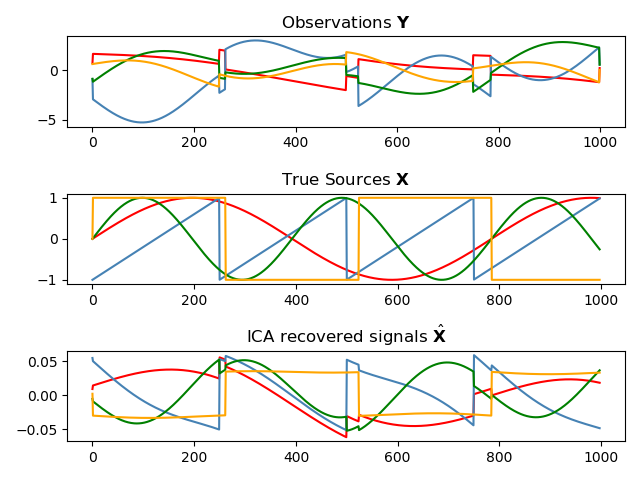
\includegraphics[scale=0.5]{figures/ICAapp/ICA_app1.png}
	\caption{}
	\label{fig:appica1}
    \end{minipage} 
    \hfill
    \begin{minipage}[t]{.45\textwidth}
		\centering
		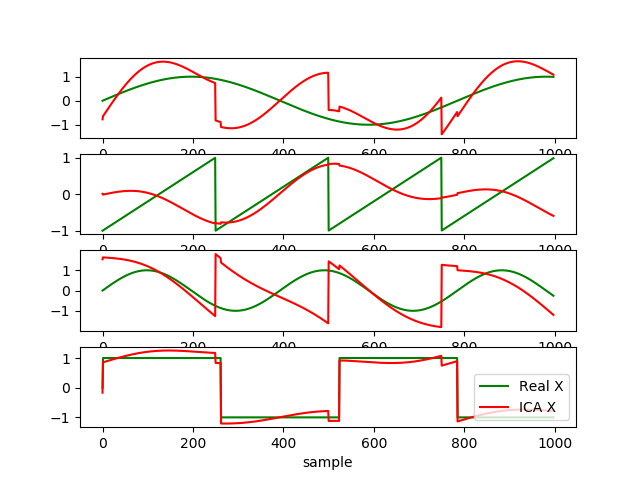
\includegraphics[scale=0.5]{figures/ICAapp/ICA_app2.png}
	\caption{}
	\label{fig:appica2}
    \end{minipage}
\end{figure}
Estimate of A is not good compare to our onw ICA. 




similar test for stochstic data, 
tjeck phase shift and A 


\begin{figure}[H]
    \begin{minipage}[t]{.45\textwidth}
		\centering
		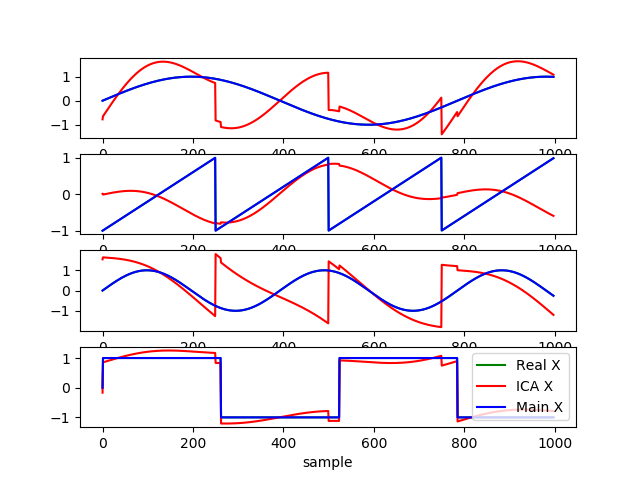
\includegraphics[scale=0.5]{figures/ICAapp/ICA_app3.png}
	\caption{}
	\label{fig:appica1}
    \end{minipage} 
    \hfill
    \begin{minipage}[t]{.45\textwidth}
		\centering
		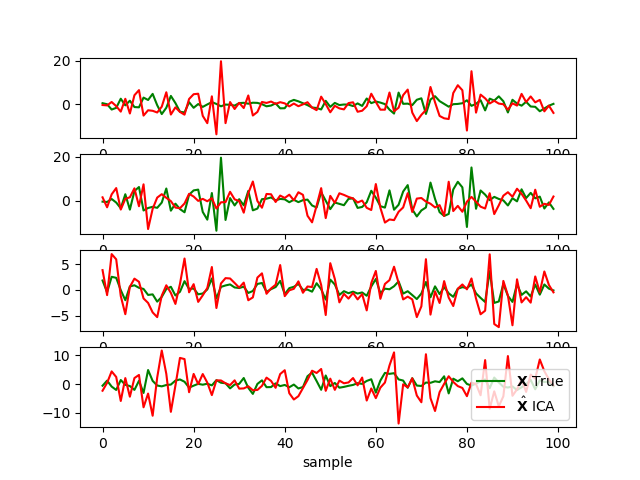
\includegraphics[scale=0.5]{figures/ICAapp/ICA_app4.png}
	\caption{}
	\label{fig:appica2}
    \end{minipage}
\end{figure}




\begin{figure}[H]
    \centering
	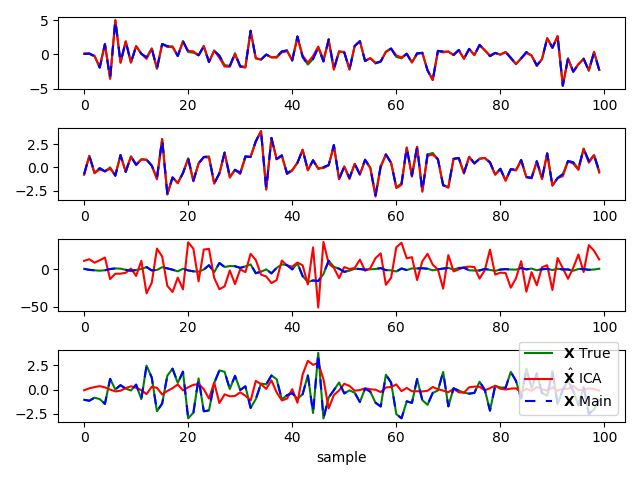
\includegraphics[scale=0.5]{figures/ICAapp/ICA_app5.png}
	\caption{MSE for system with $M=N=k=4$.}
	\label{fig:M=N_k=4}
\end{figure}  
\begin{itemize}
\item 
\end{itemize}




  


